\documentclass[a4paper]{article}

%\setlength{\parskip}{0.5\baselineskip}

\usepackage{geometry}
\geometry{left = 2.54 cm, right = 2.54 cm, top = 2.54 cm, bottom = 2.54 cm}

\usepackage{setspace}
\renewcommand{\baselinestretch}{1.0}
\usepackage{indentfirst}
\setlength{\parindent}{2em}

%\usepackage{fontspec}
%\setmainfont{Times New Roman}

\usepackage[]{cprotect}

\usepackage{hyperref}
\hypersetup{
  colorlinks=true,
  linkcolor=blue,
  filecolor=magenta,
  urlcolor=cyan,
}

\usepackage{ulem}
\usepackage{graphicx}
%\usepackage{wrapfig}
\usepackage{enumitem}
\usepackage{xcolor}
\usepackage{subcaption}
\usepackage{float}
\usepackage{amsmath, amssymb, amsthm}
\usepackage{booktabs}

\usepackage{listings} % Required for insertion of code

\lstdefinestyle{lzx}{
    % basicstyle = \small\ttfamily\fontfamily{cmr}\selectfont,
    basicstyle = \ttfamily \footnotesize,
    keywordstyle = \color{purple}\bfseries,
    % commentstyle = \color{green}\itshape,
    commentstyle = \color[RGB]{116, 153, 62}\ttfamily,
    stringstyle = \ttfamily,
    %
    tabsize = 2,
    showspaces = false,
    numberstyle = \ttfamily\color[RGB]{0,96,96},
    showstringspaces = false,
    captionpos = t,
    %
    showlines = true,
    emptylines = *2, % 2 for python, 1 for other language
    numbers = left,
    xleftmargin = 5mm,
    numbersep = 5pt,
    linewidth = \linewidth,
    % backgroundcolor=\color{red},
    frame = single,
    frameround = tttt,
    framexleftmargin = 7mm,
    %
    breaklines = true,
    postbreak = \mbox{\textcolor{red}{\( \hookrightarrow \)}\space},
}

\lstset{
    style = lzx, %
}

%\pagestyle{empty} % Not showing page number

\begin{document}
\renewcommand{\thesection}{\Roman{section}}
\renewcommand{\thesubsection}{\Alph{subsection}}
\renewcommand{\thesubsubsection}{\thesubsection.\arabic{subsubsection}}
\renewcommand{\d}{\: \mathrm{d}}
\newcommand{\e}{\mathrm{e}}

\begin{center}
  \textbf{\Large VE373 Recitation Class}\\[1em]
  \textbf{\large Week 4} \\[1em]
  2022.06.04 \\[1em]
\end{center}

\section*{L5 --- Interrupts}
  \begin{enumerate}[label = \arabic*.]
    \item \textbf{ISR --- Interrupt Service Routine}
      \par Interrupt flag should be cleared in ISR\@. Otherwise interrupt will be triggered over and over again.

      \par In ISR, you need to
      \begin{itemize}[leftmargin = 1cm]
        \item Clear interrupt flag
        \item Perhaps, stop peripheral
        \item Perhaps, disable interrupt (if in critical section)
        \item Do whatever you need to do, fix problem, respond to the peripheral
        \item Perhaps, some configuration
        \item Perhaps, restart peripheral for next interrupt
        \item Perhaps, re-enable interrupt
        \item Perhaps, start another peripheral for another interrupt
        \item Return to the interrupted instruction
      \end{itemize}

    \item \textbf{Critical section/region}
      \par Should NOT be interrupted
      \par Should disable interrupts while executing those instructions

    \item \textbf{Interrupt priority}
      \par Devices needing more urgent attention get higher priority
      \par Higher priority interrupt can interrupt execution of a lower priority interrupt

      \par Three priority levels
      \begin{itemize}[leftmargin = 1cm]
        \item Group level: 0 - 7 (highest)
        \item Subgroup level: 0 - 3 (highest)
        \item Natural level: 0 - 63 (lowest)
      \end{itemize}

    \item \textbf{Preemption}
      \par Higher priority interrupt request (IRQ) preempts (overrides) any lower priority interrupts (on group level).
      \par No preemption on subgroup and natural levels.

    \item \textbf{IPL and RIPL}
      \begin{itemize}[leftmargin = 1cm]
        \item Requested interrupt priority level (RIPL)
          \begin{itemize}[leftmargin = 1cm]
            \item In field \verb|RIPL| (\verb|CAUSE<12:10>|)
            \item 0\ldots 7, encode requested interrupt priority
          \end{itemize}
        \item Current CPU priority (IPL)
          \begin{itemize}[leftmargin = 1cm]
            \item In field \verb|IPL| (\verb|STATUS<12:10>|)
            \item Usually default 0 (no interrupt), changes to IRQ priority when servicing IRQ
            \item 0\ldots 7, encode the MIPS interrupt priority hierarchy
          \end{itemize}
        \item Preemption happens only when \verb|RIPL| \( > \) \verb|IPL|
      \end{itemize}

    \item \textbf{How to write ISR}
      \begin{lstlisting}[language = c]
#pragma interrupt foo ipl4 vector @23
void foo(void){
  ...
}
// foo will be located at the address of interrupt vector 23

#pragma interrupt bar ipl5 vector 23
void bar(void){
  ...
}
// bar will be located in general purpose program memory
// A dispatch function targeting bar will be created at exception vector address 23
    \end{lstlisting}
      \par \verb|iplx|, \verb|x| = 0\ldots 7, 0 means interrupt disabled. \verb|x| must match the group interrupt priority level specified in \verb|IPCx.|
      \par Each interrupt vector has 8 words, usually holding dispatch function that associates the vector address with the real interrupt handler function.

    \item \textbf{Change Notice (CN)}
      \par Generate interrupt upon change of state on selected CN pins
      \begin{itemize}[leftmargin = 1cm]
        \item CN pins must be configured as inputs
        \item Two adjacent reads (delayed by \verb|SYSCLK|) of CN PORT are compared, mismatch generated if different
        \item Any mismatch provides an interrupt signal
      \end{itemize}
    \item \textbf{CN configuration}
      \begin{enumerate}[label = \arabic*.]
        \item Disable all interrupts
        \item Set selected CN pin as input
        \item Enable CN module (\verb|CNCON.ON = 1|)
        \item Enable individual CN inputs, and pull ups (optional)
        \item \textcolor{magenta}{Read corresponding PORT registers to clear pre-existing mismatch condition}
        \item Configure the CN interrupt priority
        \item Clear CN interrupt flag
        \item Enable CN interrupt
        \item Enable all interrupts
      \end{enumerate}

    \item \textbf{CN ISR}
      \begin{enumerate}[label = \arabic*.]
        \item Temporarily disable CN interrupt
        \item \textcolor{magenta}{PORT should be read to clear mismatch condition}
        \item Interrupt flag should be cleared by user program
        \item \textcolor{magenta}{Current PORT value should be compared with the last PORT value of the same pin to determine which CN pin changed}
        \item Re-enable CN interrupt
      \end{enumerate}

      \par Note:
      \begin{enumerate}[label = \arabic*.]
        \item CN interrupt is a persistent interrupt: only clearing IF flag is not enough, must clear the corresponding condition.
        \item CN interrupts of all pins go into the same vector address (vector number 26). Therefore in ISR we should check which IO pin is changed.
      \end{enumerate}


  \end{enumerate}

\section*{L6 --- Liquid-Crystal Display (LCD) Driver}
  \begin{enumerate}[label = \arabic*.]
    \item \textbf{Make good use of datasheet}
      \par The datasheet of LCD is file \verb|lcd1602a_398762.pdf| in \verb|./Reference_Materials/PIC32 Starter Kit/|.

    \item \textbf{LCD module}
      \begin{figure}[H]
        \centering
        \begin{subfigure}[b]{0.6\linewidth}
          \centering
          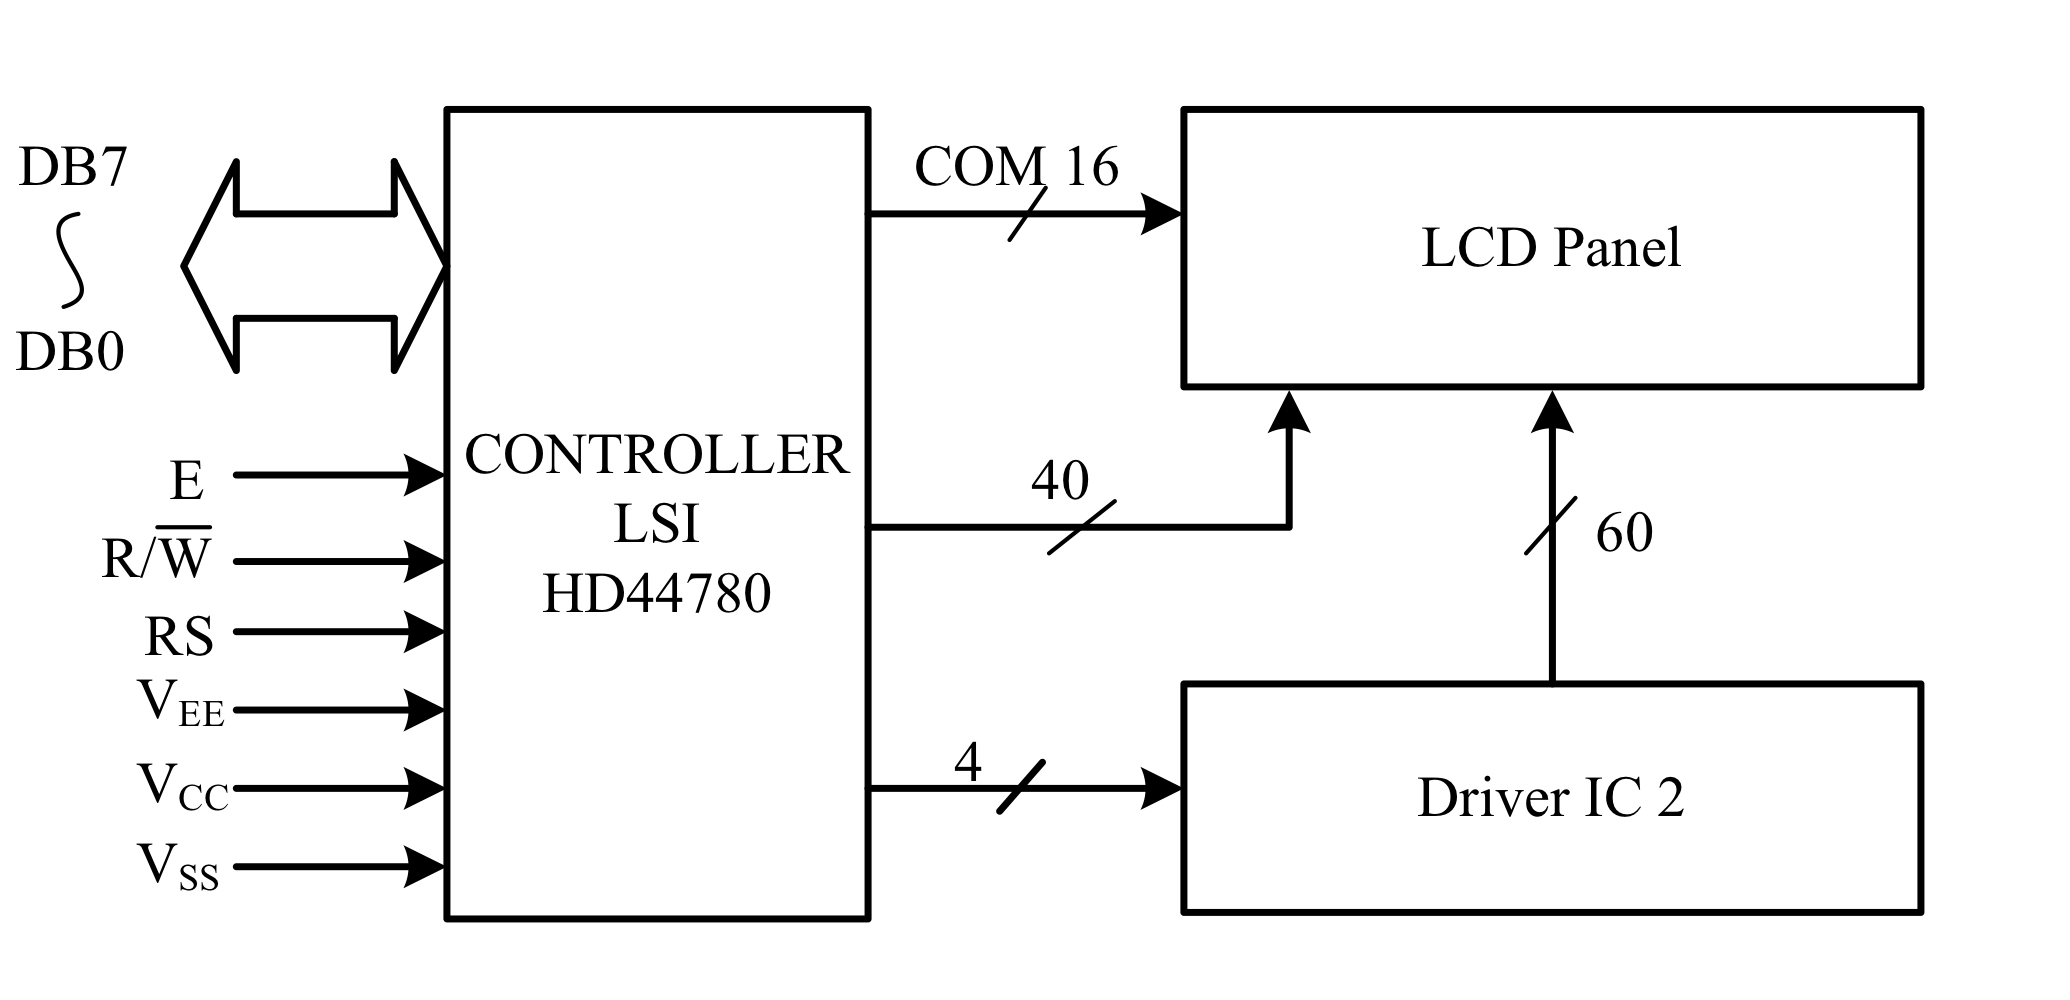
\includegraphics[width=0.9\linewidth]{LCD_module.jpeg}
          \caption{LCD module}
          \label{subfig:LCD_module.jpeg}
        \end{subfigure}
        \begin{subfigure}[b]{0.3\linewidth}
          \centering
          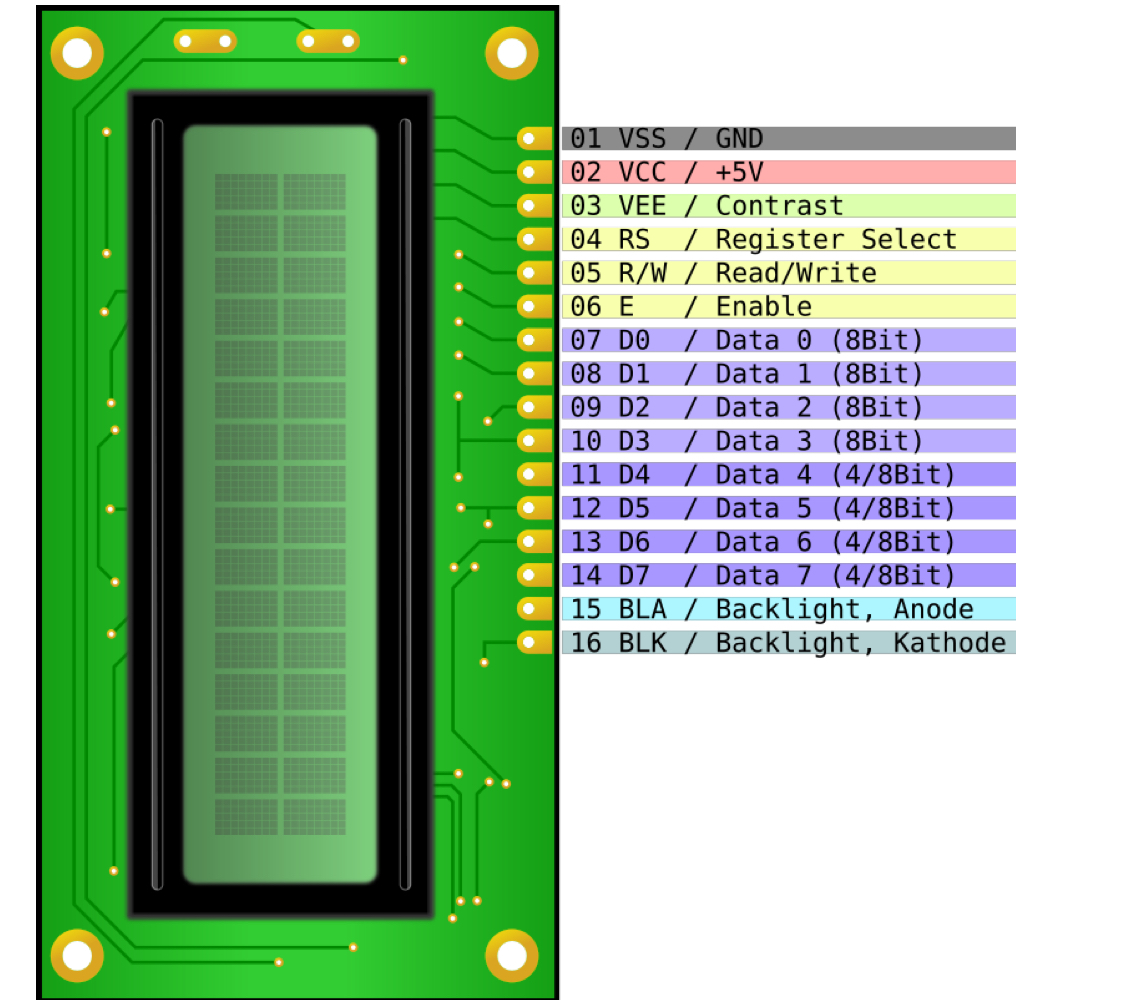
\includegraphics[width=0.9\linewidth]{LCD_pins_definition.jpeg}
          \caption{LCD pins definition}
          \label{subfig:LCD_pins_definition.jpeg}
        \end{subfigure}
        \label{fig:LCD_module}
      \end{figure}

    \item \textbf{Display Data RAM (DDRAM)}
      \begin{itemize}[leftmargin = 1cm]
        \item Can hold up to 80 bytes (characters)
        \item 40 locations mapped to Line1: \verb|0x00 - 0x27|
        \item 40 locations mapped to Line2: \verb|0x40 - 0x67|
        \item 2 line \( \times \) 16 display window is aligned with DDRAM from the head
          \begin{figure}[H]
            \centering
            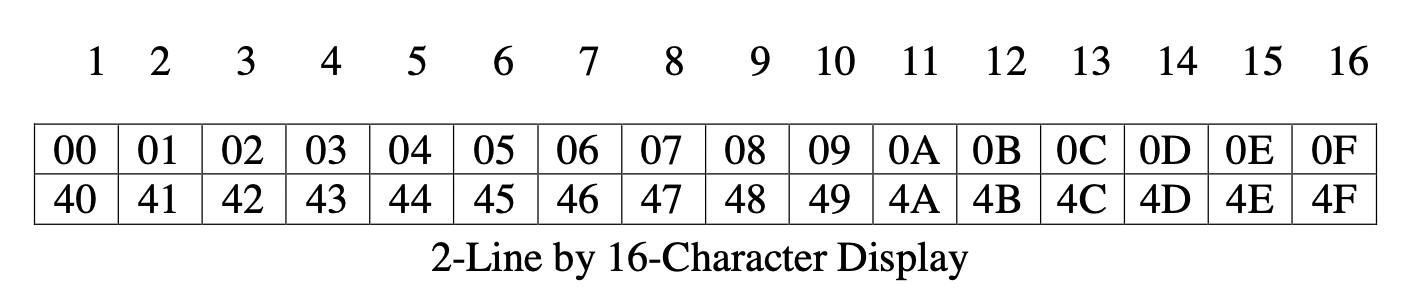
\includegraphics[width=0.6\linewidth]{Display_window.png}
            \label{fig:Display_window.png}
          \end{figure}
        \item Display window can be shifted left or right
      \end{itemize}

    \item \textbf{Code Generate ROM (CGROM)}
      \par It can be understood as the 8-bit encoding of actual character patterns. Almost the same as ASCII chart except some characters.

    \item \textbf{Control Inputs}
      \begin{itemize}[leftmargin = 1cm]
        \item RS, R/W
          \begin{figure}[H]
            \centering
            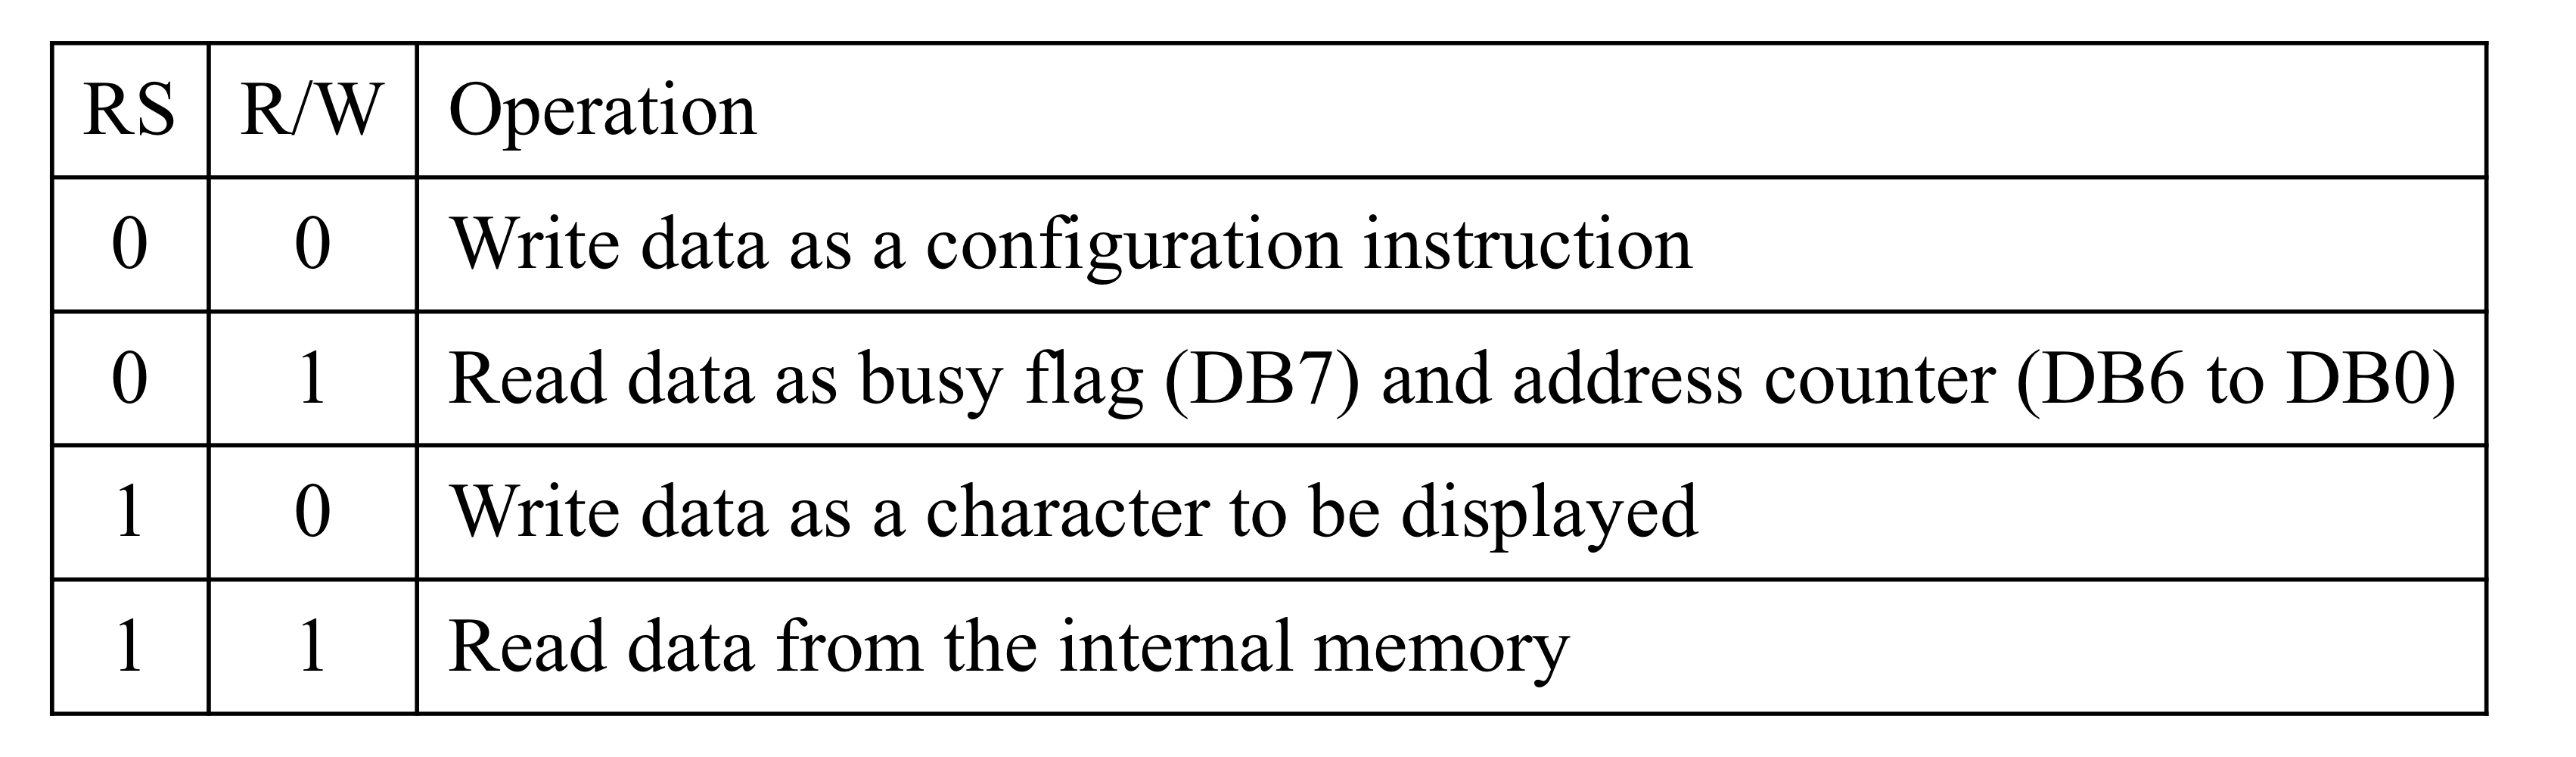
\includegraphics[width=0.6\linewidth]{RS_RW_definition.jpeg}
            \label{fig:RS_RW_definition.jpeg}
          \end{figure}
        \item E -- data transfer enable
          \par a High to Low transition on E enables the data transfer
      \end{itemize}

    \item \textbf{Instruction table}
      \par Defines the inputs to perform specific instruction. Refer to the datasheet.

    \item \textbf{Timing requirements}
      \begin{itemize}[leftmargin = 1cm]
        \item Important, must be satisfied.
        \item All instruction execution time must be satisfied, except
          \begin{itemize}[leftmargin = 1cm]
            \item For 4-bit interface, two consecutive writes, one for high nibble, one for low nibble, need no delay in between, but need 40 \( \mu \)sec after
            \item read instruction needs no time
          \end{itemize}
        \item Each write operation is enabled by a high to low transition on E input
          \par including the two consecutive nibble write
      \end{itemize}

    \item \textbf{Initialization}
      \begin{figure}[H]
        \centering
        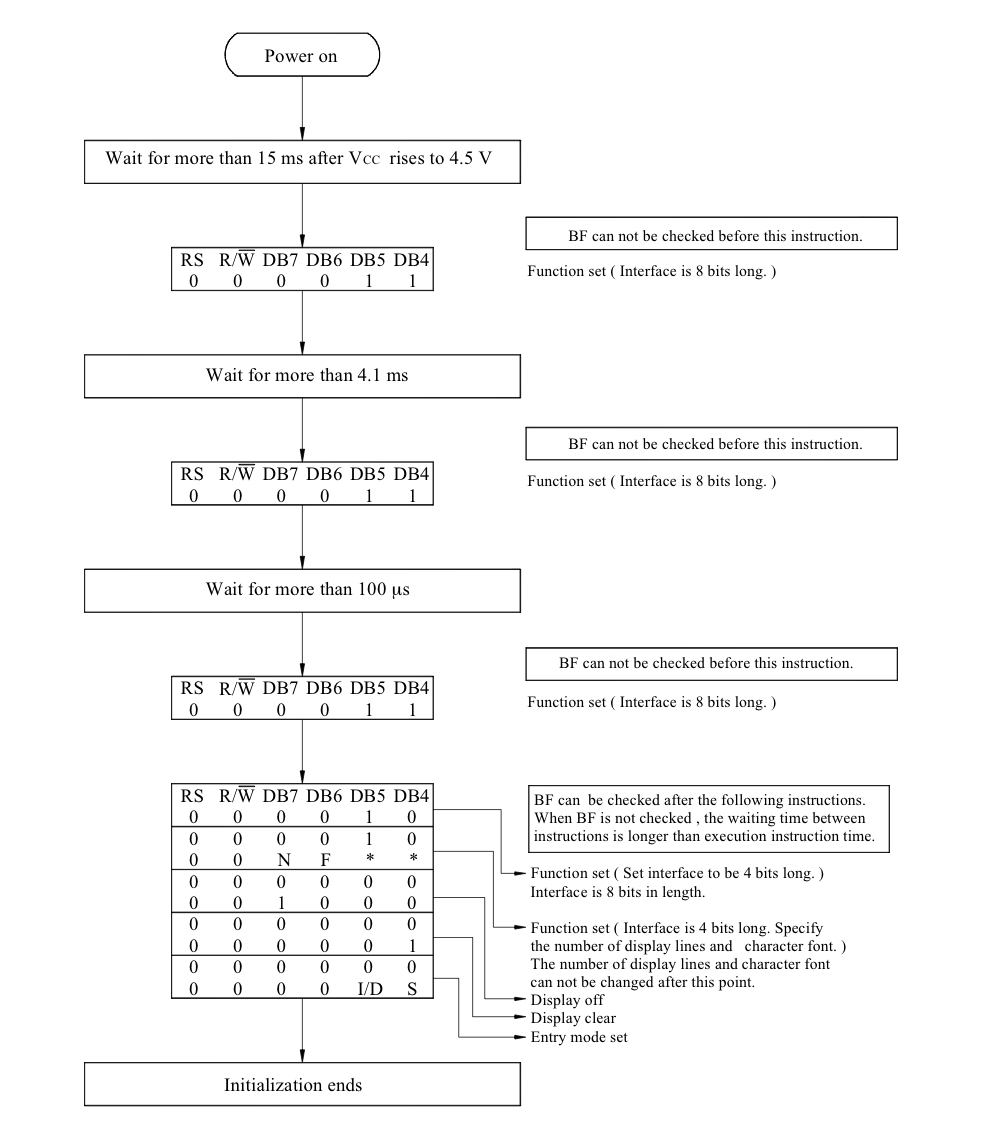
\includegraphics[width=0.9\linewidth]{LCD_config_4bit_step.jpeg}
        \caption{LCD 4-bit interface initialization}
        \label{fig:LCD_config_4bit_step.jpeg}
      \end{figure}

    \item \textbf{Tips}
      \begin{itemize}[leftmargin = 1cm]
        \item This chapter mainly focuses on the usage of LCD\@. Not much concepts.
        \item The usage of LCD will cover using timer and interrupt to generate delays, and using GPIO to communicate with LCD\@.
        \item The corresponding lab will be the first hardcore lab you meet in this course.
        \item You may have to debug your program for quite loooooong time. Start early.
      \end{itemize}
  \end{enumerate}

\section*{L7 --- Power-saving Operations}
  \begin{enumerate}[label = \arabic*.]
    \item \textbf{Static/Dynamic power}
      \par Dynamic power is comprised of switching and short-circuit power.
      \par Static power is comprised of leakage, or current that flows through the transistor when there is no activity.
      \begin{equation*}
        \begin{aligned}
          P_{\text{dynamic}} & = C V^2 f             \\
          P_{\text{static}}  & = V I_{\text{static}} \\
        \end{aligned}
      \end{equation*}

    \item \textbf{Reduce power consumption}
      \begin{itemize}[leftmargin = 1cm]
        \item Reduce operation frequency (lower frequency, lower power consumption)
        \item Halt CPU or disable peripheral modules
      \end{itemize}

    \item \textbf{9 power saving modes}
      \begin{itemize}[leftmargin = 1cm]
        \item CPU running
          \begin{itemize}[leftmargin = 1cm]
            \item FRC RUN mode: CPU uses \verb|FRC| clock source
            \item LPRC RUN mode: CPU uses \verb|LPRC| clock source
            \item SOSC RUN mode: CPU uses \verb|SOSC| clock source
            \item Peripheral bus scaling mode: \verb|PBCLK| is fraction of \verb|SYSCLK|
          \end{itemize}

        \item CPU halted
          \begin{itemize}[leftmargin = 1cm]
            \item SLEEP mode: anything using \verb|SYSCLK| (CPU and peripherals) halted, peripheral using other clock source are operating – lowest power consumption
            \item POSC IDLE mode: Primary Oscillator
            \item FRC IDLE mode: Fast RC Oscillator (8 MHz)
            \item LPRC IDLE mode: Low-Power RC Oscillator (32 KHz)
            \item SOSC IDLE mode: Secondary Oscillator (32.768 KHz)
          \end{itemize}
      \end{itemize}

    \item \textbf{SLEEP mode}
      \begin{itemize}[leftmargin = 1cm]
        \item Characteristics
          \par CPU and most peripherals are halted
          \par System clock source is shut down
          \par Lowest power consumption
          \par Several peripherals alive to wake up CPU
        \item Enter SLEEP mode
          \par \verb|SLPEN| (\verb|OSCCON<4>|) bit set, followed by “wait” assembly instruction
        \item Exit sleep mode (wake up)
          \par By these events
          \begin{itemize}[leftmargin = 1cm]
            \item Interrupt from operating peripheral
            \item Watch dog timer
            \item Reset
          \end{itemize}
          \par \textcolor{magenta}{May need start-up delay}
          \begin{itemize}[leftmargin = 1cm]
            \item Program not start running until clock signal detected stable
            \item May report fail if delay is too long
          \end{itemize}
        \item Example
          \begin{lstlisting}[language=c]
SYSKEY = 0x0;            // Write invalid key to force lock
SYSKEY=0xAA996655;       // write Key1 to SYSKEY
SYSKEY=0x556699AA;       // Write Key2 to SYSKEY
OSCCONSET = 0x10;        // Set power-saving mode as SLEEP
SYSKEY = 0x0;            // Write invalid key to force lock

asm volatile ("wait");   // Put device in selected power-saving mode
                         // code execution will resume here after
                         // wake and the ISR is complete.
                         // "volatile" forces instruction location in
                         // the program

...user code after wake-up...
        \end{lstlisting}
      \end{itemize}

    \item \textbf{IDLE mode}
      \begin{itemize}[leftmargin = 1cm]
        \item CPU is halted
          \begin{itemize}[leftmargin = 1cm]
            \item System clock source is still running
            \item Peripherals alive, unless individually configured to halt when in IDLE
            \item \textcolor{magenta}{Low start-up latency}
            \item Operating clock frequency may be slowed down to reduce power consumption
          \end{itemize}
        \item Enter IDLE mode
          \par \verb|SLPEN| (\verb|OSCCON<4>|) bit cleared followed by “wait” assembly instruction, e.g.  \\
          \verb|OSCCONCLR = 0x10; asm ("wait");|
        \item Exit from IDLE mode
          \begin{itemize}[leftmargin = 1cm]
            \item Interrupt from operating peripheral
            \item Watch dog timer
            \item Reset
          \end{itemize}
      \end{itemize}

    \item \textbf{Wake-up CPU}
      \begin{itemize}[leftmargin = 1cm]
        \item Peripheral interrupt
          \begin{itemize}[leftmargin = 1cm]
            \item If current CPU priority is greater (IPL \( > \) RIPL), CPU remains halted
              \par System remains IDLE, or system enters IDLE from SLEEP
            \item If requested peripheral IRQ priority is greater (RIPL \( > \) IPL)
              \par CPU services IRQ, then continues executing instruction following “wait”
          \end{itemize}

        \item WDT (watch dog timer) Non-Maskable Interrupt (NMI)
          \begin{figure}[H]
            \centering
            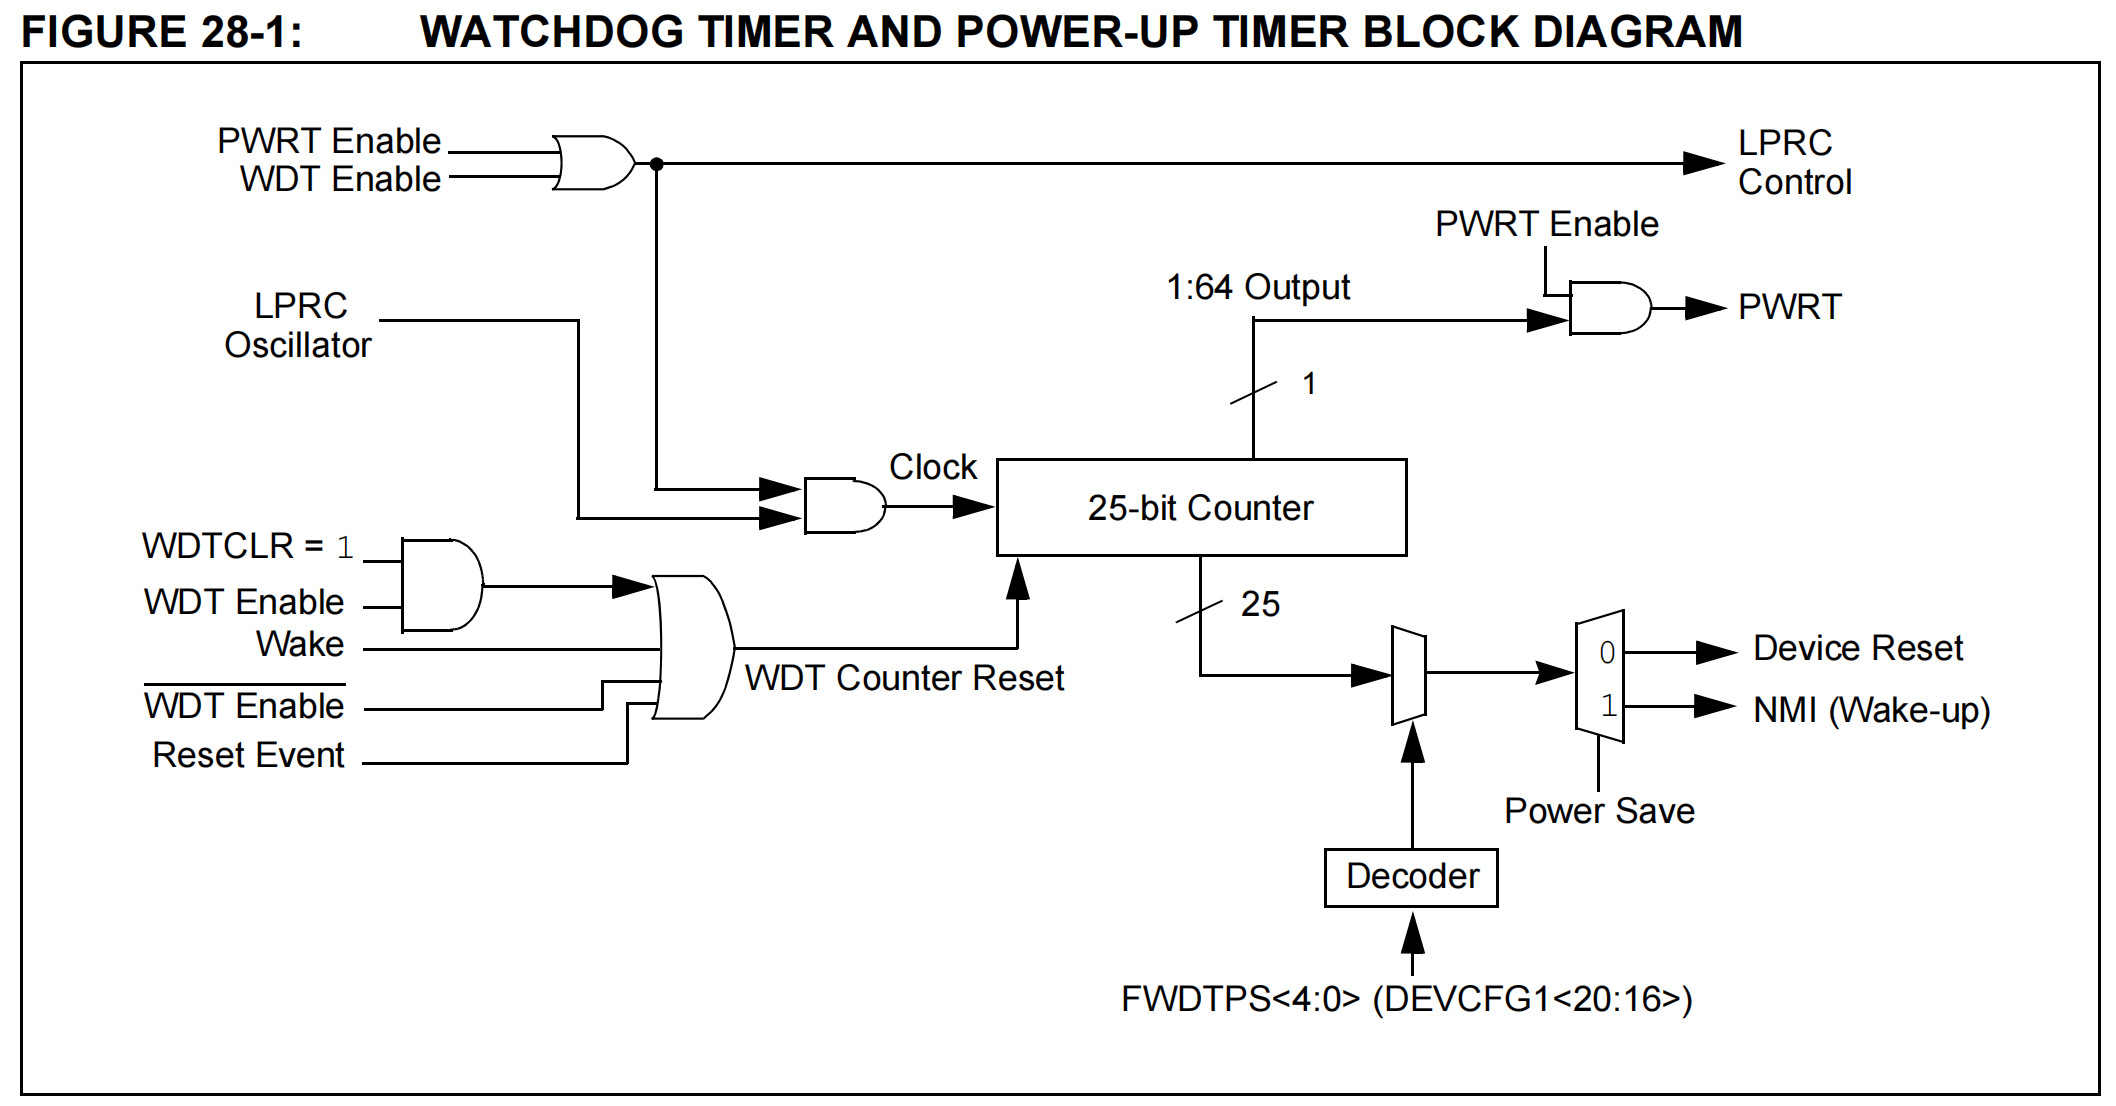
\includegraphics[width=0.8\linewidth]{Watch_dog_timer_block_diagram.png}
            \label{fig:Watch_dog_timer_block_diagram.png}
          \end{figure}

          \par Also used to check software malfunction. Error if software not periodically clear WDT
      \end{itemize}

  \end{enumerate}


\end{document}